\section{Neubewertung des Randwertproblems}
Ein zentrales Problem bei der Analyse von topografischen Daten in begrenzten Kartenausschnitten ist das Randwertproblem. Es entsteht, weil die topografischen Informationen an den Grenzen des Datensatzes enden und somit eine vollständige Analyse der Umgebung für Punkte in Randnähe unmöglich ist. Ein Hang, der in den Kartenausschnitt hineinragt, könnte fälschlicherweise als eigenständiger Berg klassifiziert werden, da der Algorithmus nicht erkennen kann, dass es sich lediglich um den Ausläufer eines außerhalb liegenden, höheren Berges handelt. Der höchste Punkt dieses Hangs innerhalb des Ausschnitts würde fälschlicherweise als Gipfel identifiziert.

Um dieses Problem systematisch zu adressieren, wird die Konzepte der \textit{minimalen Prominenz} und \textit{minimalen Dominanz} eingeführt. Diese Metriken quantifizieren die untere Schranke für die wahren Prominenz- und Dominanzwerte, die allein aus den Daten des Kartenausschnitts herleitbar ist. Sie repräsentieren eine konservative Schätzung unter der Annahme, dass sich direkt außerhalb der Kartengrenze eine unendlich hohe Bergkette befindet.

\begin{figure}[h]
    \centering
    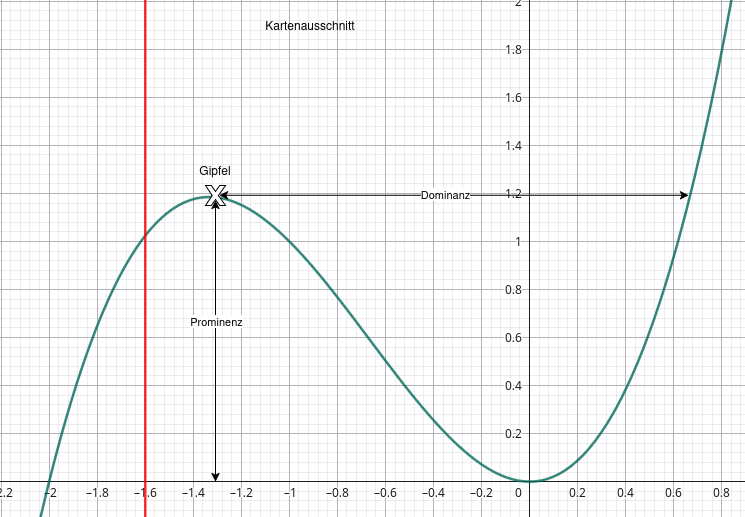
\includegraphics[width=1.0\textwidth]{Diagramms/Dominanz_Prominenz_2D.drawio.png}
    \caption{2D-Geländeprofil zur Illustration von Prominenz und Dominanz eines Gipfels}
    \label{fig:Geländeprofil_prominenz_dominanz}
\end{figure}

Die Abbildung \ref{fig:Geländeprofil_prominenz_dominanz} zeigt die reguläre Berechnung von Prominenz und Dominanz in einem idealisierten, unbegrenzten Gelände. Die Dominanz ist der Abstand zum nächstgelegenen höheren Punkt, und die Prominenz ist die Höhendifferenz zum maßgeblichen Sattel.

\begin{figure}[h]
    \centering
    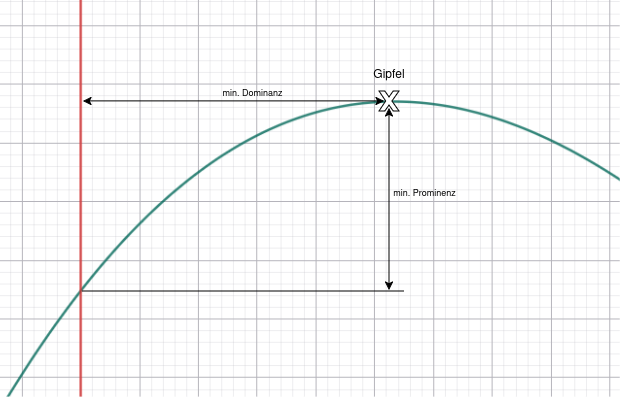
\includegraphics[width=1.0\textwidth]{Diagramms/min_Dominanz_Prominenz_2D.drawio.png}
    \caption{2D-Geländeprofil zur Illustration der minimalen Prominenz und Dominanz bei begrenztem Kartenausschnitt.}
    \label{fig:Geländeprofil_min_prominenz_dominanz}
\end{figure}

Wird das Gelände jedoch durch einen Kartenausschnitt begrenzt, wie in Abbildung \ref{fig:Geländeprofil_min_prominenz_dominanz} dargestellt, ändern sich die garantierbaren Werte. Die minimale Dominanz wird als das Minimum aus zwei Werten definiert: der innerhalb des Ausschnitts berechneten Dominanz und der direkten Distanz des Gipfels zum Kartenrand. Diese Metrik wurde eingeführt, da ein höherer Punkt unmittelbar außerhalb des sichtbaren Kartenbereichs existieren könnte, was die wahre Dominanz limitieren würde. Analog dazu ergibt sich die minimale Prominenz als das Minimum aus der regulär berechneten Prominenz und der Höhendifferenz des Gipfels zum höchsten Sattel, der zum Kartenrand führt. Dieser "Randsattel" repräsentiert den höchsten Punkt, der mindestens überwunden werden muss, um den Kartenausschnitt zu verlassen, und begrenzt somit die nachweisbare Prominenz. Diese Werte sollen zeigen in wie aussagekräftig der aus dem kartenausschnitt errechnete Dominanz- und Prominenzwert ist. \todo{falls in ui verwendet: Sicherheitswert in Prozent der Berechnugn der Dominaz und Prominenz}

Theoretsich lässt sich so auch der pauschale Ausschluss von Werten innerhalb eines Randabstands anders beschreiben. Der Randabstand von $x$~Pixeln lässt sich in die Bedingung, dass die minimale Dominanz kleiner ist als das Produkt aus $x$ und der Bodenauflösung (in Meter pro Pixel) ist umformulieren. Dies wird jedoch im Algorithmus umgesetzt, weil dadurch Randfälle wie zum Beispiel ein größerer Randabstand als Dominanzgrenzwert berücksichtig werden müssten. Im Algorithmus wird weiterhin mit einem pixelbassierten Abstand gerechnet. 

Es wurde untersucht in wie weit es die Laufzeit senkt anstatt bei der Bestimmung der lokalen Hochpunkte anstatt der Setzung aller Randwertpunkte auf 0 eine Possitionsbassierte Schranke zu verwenden, die alle Gipfel aussortiert,d ie sich im Randbereich befinden. Nach mehreren Tests ist hier jedoch keine Verbesserung der Laufzeit erkennbar gewesen. Daher wurde der alte übersichtlichere und erprobte Ansatz weiter verwendet. 

Eine alternative Implementierung des Randwertbereichs wäre auf Basis der minimalen Prominenz und Dominanz. Dabei würde alle Gipfel aussortiert werden, deren minimale Prominenz oder Dominanz unter dem jeweiligen Schwelenwert liegt. Diese Methode der Randwertbehandlung ist für diesen Algorithmus nicht zielführend, da dadurch mehr falschnegative Werte entstehen, die wir eigentlich verhindern wollen. Darum wurde sie auch nicht implementiert.

Um das Problem der Gipfel am Kartenrand zu lösen musste an einer anderen Stelle angesetzt werden. Es hat sich herausgestellt, dass wenn der Randbereich auf Null gesetzt wird und nun auf genau diesen Geodaten eine Prominenzberechung durchgeführt wird die Daten alle Werte im Randbereich ignorieren, was nicht der Sinn des Randwertes ist (wie in \ref{fig:randwert_problem_1}). Der Randwert sollte eigentlich einen Puffer geben, damit die Prominenz und die Dominanz besser berechnet werden können und nicht den Kartenbereich ohne Vorteil verkleinern.  

\begin{figure}[h]
    \centering
    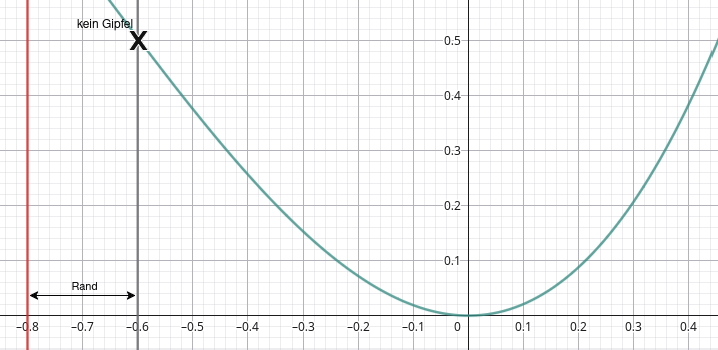
\includegraphics[width=1.0\textwidth]{Diagramms/Randwert_Problem_1.drawio.png}
    \caption{2D-Geländeprofil zur Illustration der minimalen Prominenz und Dominanz bei begrenztem Kartenausschnitt.}
    \label{fig:randwert_problem_1}
\end{figure}

\begin{figure}[h]
    \centering
    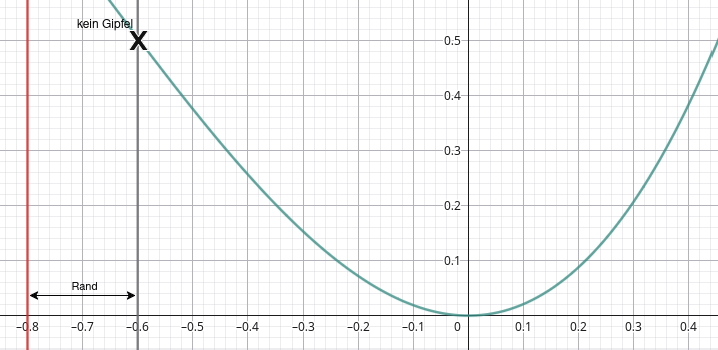
\includegraphics[width=1.0\textwidth]{Diagramms/Randwert_Problem_2.drawio.png}
    \caption{2D-Geländeprofil zur Illustration der minimalen Prominenz und Dominanz bei begrenztem Kartenausschnitt.}
    \label{fig:randwert_problem_2}
\end{figure}

Wenn nun jedoch die ursprünglichen Geodaten zur Prominenz und Dominanzbestimmung verwendet werden, werden die Gipfel auf dem Kartenrand nicht mehr falsch entdeckt (\ref{fig:randwert_problem_2}). 